\documentclass[]{revdetua}
\usepackage{graphicx}
\usepackage{float}

\begin{document}

\Header{Volume}{1}{Novembro}{2022}{0}
% Note: the month must be in Portuguese

\title{Advanced Algorithms First Project \linebreak Maximum Cut Problem}
\author{Daniela Dias 98039}
\maketitle

\begin{abstract}
This report presents algorithmic solutions for the Maximum Cut Problem, including a formal analysis of each algorithm's efficiency, a discussion of the obtained results, and predictions for large problem instances. This problem is addressed by the course "Advanced Algorithms" at the University of Aveiro. The proposed algorithms include one exhaustive search algorithm and two greedy algorithms (breadth-first search and other greedy heuristics). The chosen coding language was Python(3.10).
\end{abstract}

\begin{resumo}% Note: in Portuguese
Este relatório apresenta soluções algorítmicas para o problema Maximum Cut, incluindo uma análise formal da eficência de cada algoritmo, uma discussão dos resultados obtidos e previsões para problemas de maior escala. Este problema é abordado pelo curso "Algoritmos Avançados" na Univerdade de Aveiro. Os algoritmos propostos incluem uma algoritmo de pesquisa exaustiva e dois algoritmos gulosos (pesquisa em largura e outras heurísticas). A linguagem de programação escolhida foi o Python(3.10).
\end{resumo}

\begin{keywords}% Note: in English (optional)
Graph, Cut, Cut Set, Maximum Cut, Vertices, Edges, Exhaustive Search, Greedy, Heuristics
\end{keywords}

\begin{palavraschave}% Note: in Portuguese (optional)
Grafo, Cut, Cut Set, Maximum Cut, Vértices, Arestas, Pesquisa Exaustiva, Algoritmos Gulosos, Heurísticas
\end{palavraschave}

\section{Introduction}
This report addresses the first project of "Advanced Algorithms". For this project, we design and test an exhaustive search algorithm to solve the Maximum Cut problem, as well as other methods using greedy heuristics.

The following sections describe the problem in detail, explain the added optimizations (in particular, with handling graphs), and analyze the computational complexity of the developed algorithms. For this analysis, we perform a formal and experimental computational complexity analysis of the algorithms. The later includes a series of experiments for progressively larger problem instances to register and study the number of basic operations carried out, the number of solutions tested, and the execution time. Finally, we compare the results of both the formal and experimental analyses.

With the report, we submitted the code files and the results files (from the execution of all the algorithms). To run the code, first generate the graphs, then run the chosen algorithm file:\linebreak

\$ python generate\_graphs.py 

\$ python exhaustive\_search.py

\$ python breadth\_first\_search.py

\section{Maximum Cut Problem}

This report handles the Maximum Cut Problem, which we can solve by finding the maximum cut for a given undirected graph G(V, E), with n vertices and m edges. In graph theory, a cut is a partition of the vertices of a graph into two disjoint subsets, determining a set of edges with one endpoint in each subset. These edges are said to cross the cut. A maximum cut of G is a partition of the graph's vertices into two complementary subsets S and T, such that the number of edges between the set S and the set T is as large as possible. 

In the context of the problem, it's relevant to evaluate the characteristics of the graphs and their structure. The graph instances used in the computational experiments represent the following scenario:
\begin{itemize}
\item Graph vertices are 2D points on the XoY plane, with integer-valued coordinates between 1 and 20.
\item Graph vertices should neither be coincident nor too close.
\item The number of edges sharing a vertex is randomly determined.
\item Use 12.5\%, 25\%, 50\%, and 75\% of the maximum number of edges for the number of vertices.
\item Graph edges are unweighted and undirected.
\end{itemize}

Since the number of edges can be significantly smaller than the number of vertices (when generating the graph instances, we use 12.5\% and 25\% of the maximum number of edges for the number of vertices), we can confirm that the generated graphs aren't all connected. A connected graph is a graph linked in the sense of a topological space: there is a path from any point to any other point in the graph (an edge connecting all vertices). A graph that is not connected is said to be disconnected.

This matters to our problem for the following reasons:
\begin{itemize}
\item The cut set must result in a partition of the vertices into two non-empty disjoint subsets.
\item Vertices without edges have zero impact in a cut set (the number of edges crossing the cut doesn't change).
\end{itemize}

Hence, we were able to implement optimizations that restricted the problem to a smaller version (subset) of the problem. Instead of working with the complete graph, we work with a subgraph of the initial graph, ignoring vertices without edges (with a degree equal to zero). This optimization decreases the computational complexity of the problem.

The first step to constructing a graph is generating the list of vertices and edges. The list of vertices is a list of randomly generated tuples of coordinates with 2, 4, 8, 16, 32, 62, 128, and 256 vertices (numbers by the power of 2). The coordinates take values between 1 and 20, inclusive. Since the graph is undirected in this context, the list of edges is a list of the tuples of the vertices involved  (their coordinates). Consequently, (x1, x2) is the equivalent of (x2, x1). Following are the examples of generated vertices and edges:

\begin{itemize}
\item Vertices: [(5, 3), (12, 15), (11, 19), (3, 17)]
\item Edges: [((3, 17), (11, 19)), ((12, 15), (3, 17)), ((5, 3), (3, 17)), ((12, 15), (5, 3))]
\end{itemize}

To enable the storage of graphs (in JSON files), we chose to identify the vertices by numeric id's and convert the graphs data in a node-link format suitable for JSON serialization and use in Javascript documents, with networkx.node\_link\_data(graph). An example, with the previous vertices and edges, would be:

\begin{itemize}
\item {"directed": false, "multigraph": false, "graph": {}, "nodes": [{"id": 0}, {"id": 1}, {"id": 2}, {"id": 3}], "links": [{"source": 0, "target": 3}, {"source": 0, "target": 1}, {"source": 1, "target": 3}, {"source": 2, "target": 3}]}
\end{itemize}

To load the graph files, we have to read the file and convert the read data with nx.node\_link\_graph(graph\_data). Finally, we identify each cut set by the vertices partition, A and B. For example:

\begin{itemize}
\item A:  [3]
\item B:  [0, 1, 2]
\end{itemize}

\section{Analysis of Algorithm Efficiency}

\subsection{Measuring an Input’s Size}

It is logical to investigate an algorithm’s efficiency as a function of some parameter n indicating the algorithm’s input size. For this case, n could be the size of the list of vertices in the generated graphs. However, since the algorithm only examines the connected vertices (with at least one edge), we measured the input size by the number of connected vertices.

\subsection{Units for Measuring Running Time}

For measuring the running time of the algorithms developed, we decided to use two units of time measurement: execution time in seconds and the number of basic operations executed by the algorithm. 

It is worth noting that the first measurement has drawbacks since it depends on the speed of the computer running the program, the implementation of the algorithm, and the compiler used in generating the machine code. On the other hand, we can objectively measure the running time by identifying a basic operation and computing the number of times this operation is executed on inputs of size n. 

The basic operation contributes the most to the total running time: it is the most time-consuming operation in the algorithm’s innermost loop. In our case, this operation corresponds to the comparison between the current maximum cut and the solution being tested. Since the comparison is executed on each repetition of the loop and the assignment (of maximum cut value) is not, we consider the comparison to be the algorithm’s basic operation. 

Since the calculations behind the value of the cut set are the same for all algorithms, we do not consider it a basic operation.

\subsection{Worst-Case, Best-Case, and Average-Case Efficiencies}

We have established that it is reasonable to measure an algorithm’s efficiency as a function of the size of the algorithm’s input. However, the running time of the same algorithm can be quite different for the same list size n. Hence, we will consider the worst-case, best-case, and average-case efficiencies when analyzing the developed algorithms.

The worst-case efficiency of an algorithm is its efficiency for the worst-case input of size n (for which the algorithm runs the longest among all possible inputs of that size). For our algorithms, the worst-case happens for the largest number of cut set comparisons among all possible inputs of size n. This analysis provides very important information about an algorithm’s efficiency by bounding its running time from above. 

The best-case efficiency of an algorithm is its efficiency for the best-case input of size n (for which the algorithm runs the fastest among all possible inputs of that size). For our algorithms, the best-case happens for the smallest number of cut set comparisons among all possible inputs of size n.

Finally, the average-case of an algorithm is its efficiency for the "typical" (or random) case input of size n. It is the most challenging to calculate.

\section{Exhaustive Search Algorithm}

The first algorithm developed was an exhaustive search algorithm capable of always finding the most optimal solution for any given graph. This is possible by calculating the cut for all possible combinations of two subsets (subgraphs) of the initial graph and obtaining the one with the maximum number of edges crossed. For the generation of all possible combinations, it is worth noting that (A: X, B: Y) is equivalent to (A: Y, B: X).

As mentioned previously, we consider the algorithm's basic operation to be the comparison between the current value of the maximum cut and the value of the cut set being tested. Since we calculate the cut for all possible combinations of two subsets of the initial graph, no matter if the maximum cut has already been found, the number of comparisons will be the same for all inputs of size n. Therefore, there is no need to distinguish among the worst, average, and best cases. It's also worth noting that the number of solutions tested will be equal to the number of comparisons. 

This algorithm is simple but extremely costly in both time and space complexity. To obtain its computational complexity, we only need to consider the number of cut comparisons, equivalent to the number of vertices partitions generated and tested (the algorithm makes one comparison on each execution of the loop, repeating for every single partition). Since the generation of all combinations creates 2**n partitions, the computational complexity is 2**n (n being the number of vertices with edges). We can conclude that the algorithm's order of growth is exponential, and larger problem instances will result in a quickly rising number of iterations.

The exhaustive algorithm was unable to solve the Maximum Cut problem with more than 16 nodes, failing to finish its execution in less than 60 seconds. Without the timeout, its execution throws a MemoryError due to a lack of memory.

\section{Greedy Algorithm}

The second algorithm developed was a greedy algorithm. It's a local search algorithm that maintains a candidate cut and iteratively makes it better and better via small, local modifications. It goes as follows:
\begin{itemize}
\item Let (A, B) be an arbitrary cut of G, and start with all vertices in the subset A.
\item While there is a vertex that increases the value of the cut set (i.e. increases the number of crossing edges) by moving from subset A to subset B, and vice-versa, move the vertex to that subset.
\item When there is no possible improvement, return the final cut (A, B).
\end{itemize}

The algorithm's basic operation is the comparison between the current value of the maximum cut and the value of the cut set being tested. Here, for each iteration, we complete two comparisons: If the cut is greater with a given vertex in one subset than in the other and if the new partition (with the vertex moved) increases the current cut. Since we consider one solution at a time until we find a (possibly local) maximum cut, the number of comparisons will differ for all inputs of size n. Hence, we should evaluate the worst, average, and best cases, in particular, the worst and best cases.

The algorithm performs poorly (time and space-wise) and doesn't guarantee to return the maximum cut due to the existence of local optima. However, it promises a good worst-case performance guarantee and always outputs a cut in which the number of crossing edges is at least 25\% of the maximum possible. To obtain its computational complexity, we need to consider the number of cut comparisons, equivalent to twice the number of vertices partitions tested (the algorithm makes two comparisons on each execution of the loop, repeating for every single partition).

We get the best case when we only need to move one vertex from a subset to another, in other words, $\Omega(n)$ = 2 (we calculate two comparisons for each iteration). However, for the worst case, we have to move all the vertices except one from subset A to subset B, meaning that $O(n)$ = 2n-1 = 2n = n. With this, we can conclude that the algorithm's order of growth is linear.

\section{Breadth-First Search}

The final algorithm also uses greedy heuristics. It is a breadth-first search algorithm that works as follows:
\begin{itemize}
\item Generate a breadth-first search tree with the initial graph and an arbitrary vertex as the root.
\item Create a subset A with the vertices in the even layers of the breadth-first search tree.
\item Create a subset B with the vertices in the odd layers of the breadth-first search tree.
\item Calculate the number of edges crossing (the cut) and return the final cut set (A, B).
\end{itemize}

Once again, the algorithm's basic operation is the comparison between the current value of the maximum cut and the value of the cut set being tested. Since we only calculate the cut for a single combination of two subsets of the initial graph (even and odd layers of a breadth-first search tree), the number of comparisons will be the same for all inputs of size n. Therefore, there is no need to distinguish among the worst, average, and best cases. It's also worth noting that the number of solutions tested will equal the number of comparisons.

Although it doesn't guarantee the correct value of maximum cut, it is the most simple and efficient algorithm of the three, with highly promising results. No matter the input size n, we only perform a single basic operation (one comparison because we only test a solution every time); hence, the computation complexity is 1. We can conclude that the algorithm's order of growth is linear (constant), and larger problem instances don't result in a rising number of iterations.

\section{Results}

\subsection{Maximum Cut}

By comparing the greedy algorithms to the exhaustive search, which obtains the maximum cut for any input of size n, we can prove that these algorithms aren't completely accurate. We can also confirm that the first greedy algorithm (local search) is extremely less correct than the second (breadth-first search). Although it has a higher accuracy for graphs up to 16 vertices (36\% accuracy), the first greedy algorithm obtains a maximum cut considerably lower than the intended. 

\begin{table}[!ht]
    \centering
    Exhaustive Algorithm
    \begin{tabular}{|l|l|l|l|}
    \hline
        Graph         & Vertices      & Edges       & Maximum Cut      \\ \hline
        4 & 2 & 1 & 1 \\ \hline
        4 & 4 & 3 & 3 \\ \hline
        4 & 4 & 4 & 3 \\ \hline
        8 & 6 & 3 & 3 \\ \hline
        8 & 7 & 7 & 6 \\ \hline
        8 & 8 & 14 & 11 \\ \hline
        8 & 8 & 21 & 15 \\ \hline
        16 & 15 & 15 & 13 \\ \hline
        16 & 16 & 30 & 23 \\ \hline
        16 & 16 & 60 & 41 \\ \hline
        16 & 16 & 90 & 56 \\ \hline
    \end{tabular}
\end{table}

\begin{table}[!ht]
    \centering
    Greedy Algorithm
    \begin{tabular}{|l|l|l|l|}
    \hline
        Graph         & Vertices      & Edges       & Maximum Cut      \\ \hline
        4 & 2 & 1 & 1 \\ \hline
        4 & 4 & 3 & 3 \\ \hline
        4 & 4 & 4 & 3 \\ \hline
        8 & 6 & 3 & 3 \\ \hline
        8 & 7 & 7 & 5 \\ \hline
        8 & 8 & 14 & 7 \\ \hline
        8 & 8 & 21 & 7 \\ \hline
        16 & 15 & 15 & 6 \\ \hline
        16 & 16 & 30 & 10 \\ \hline
        16 & 16 & 60 & 15 \\ \hline
        16 & 16 & 90 & 14 \\ \hline
    \end{tabular}
\end{table}

\begin{table}[!ht]
    \centering
    Breadth-First Search
    \begin{tabular}{|l|l|l|l|}
    \hline
        Graph         & Vertices      & Edges       & Maximum Cut      \\ \hline
        4 & 2 & 1 & 1 \\ \hline
        4 & 4 & 3 & 3 \\ \hline
        4 & 4 & 4 & 3 \\ \hline
        8 & 6 & 3 & 1 \\ \hline
        8 & 7 & 7 & 4 \\ \hline
        8 & 8 & 14 & 4 \\ \hline
        8 & 8 & 21 & 11 \\ \hline
        16 & 15 & 15 & 8 \\ \hline
        16 & 16 & 30 & 17 \\ \hline
        16 & 16 & 60 & 35 \\ \hline
        16 & 16 & 90 & 38 \\ \hline
    \end{tabular}
\end{table}

\subsection{Basic Operations}


\begin{figure}[H]
    \centering
    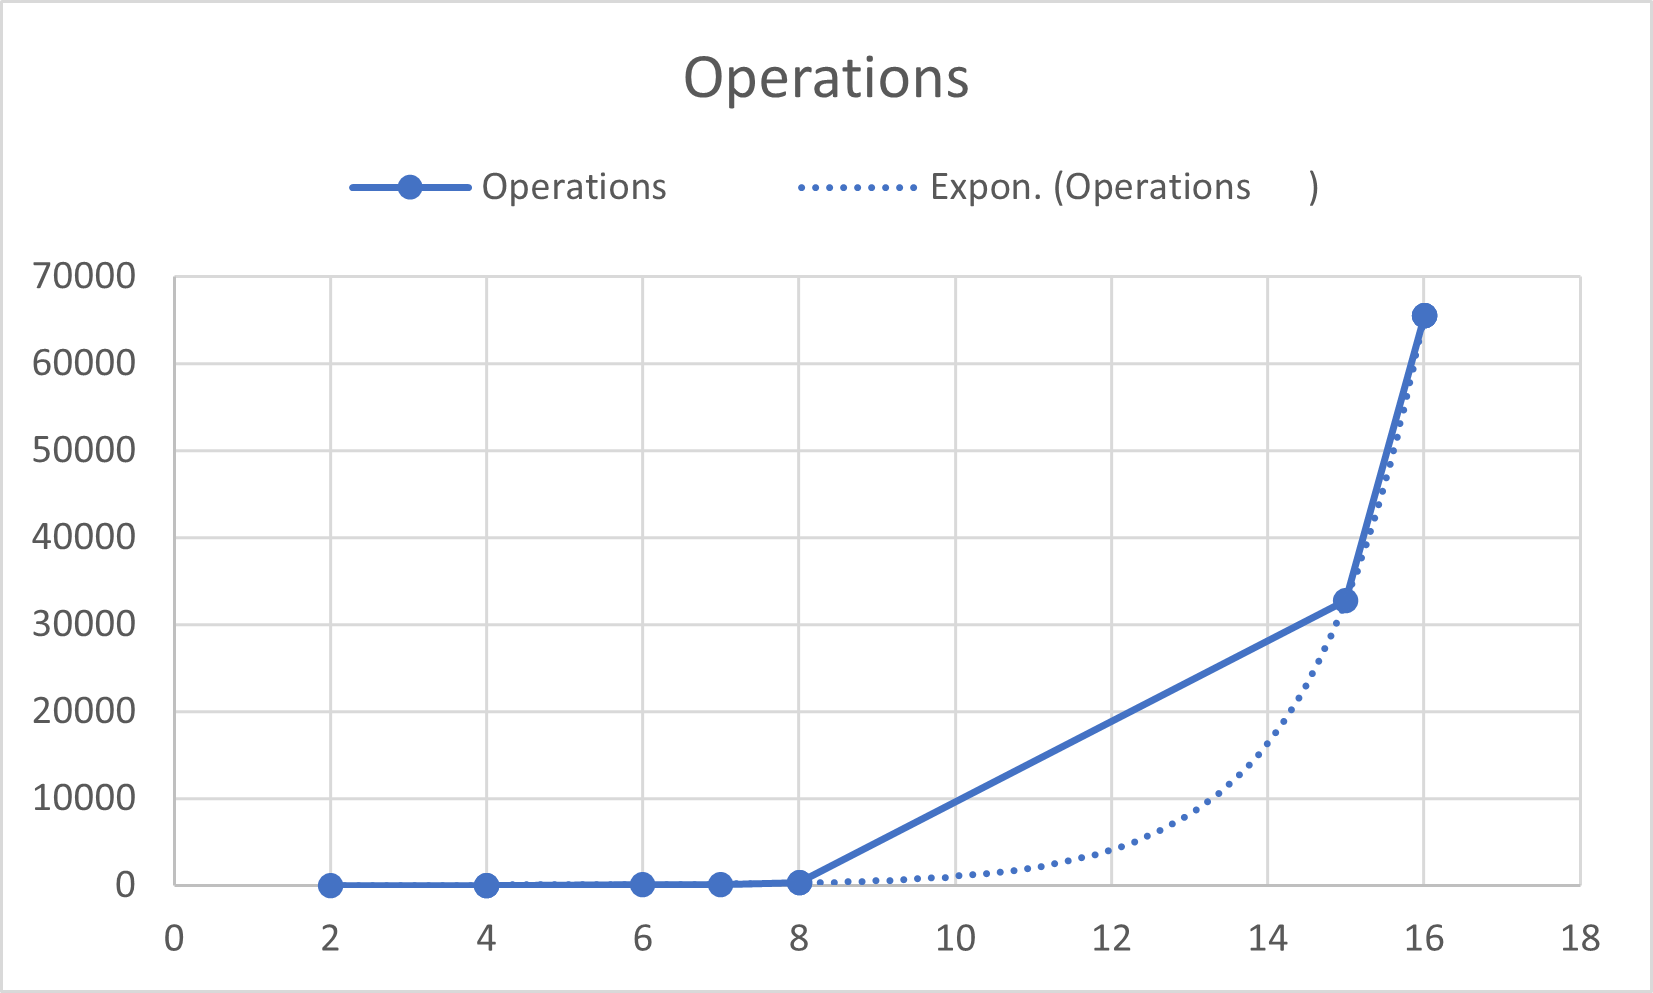
\includegraphics[width=8cm]{Exhaustive Search/Operations.png}
    \caption{Exhaustive Search Basic Operations}
\end{figure}

\begin{figure}[H]
    \centering
    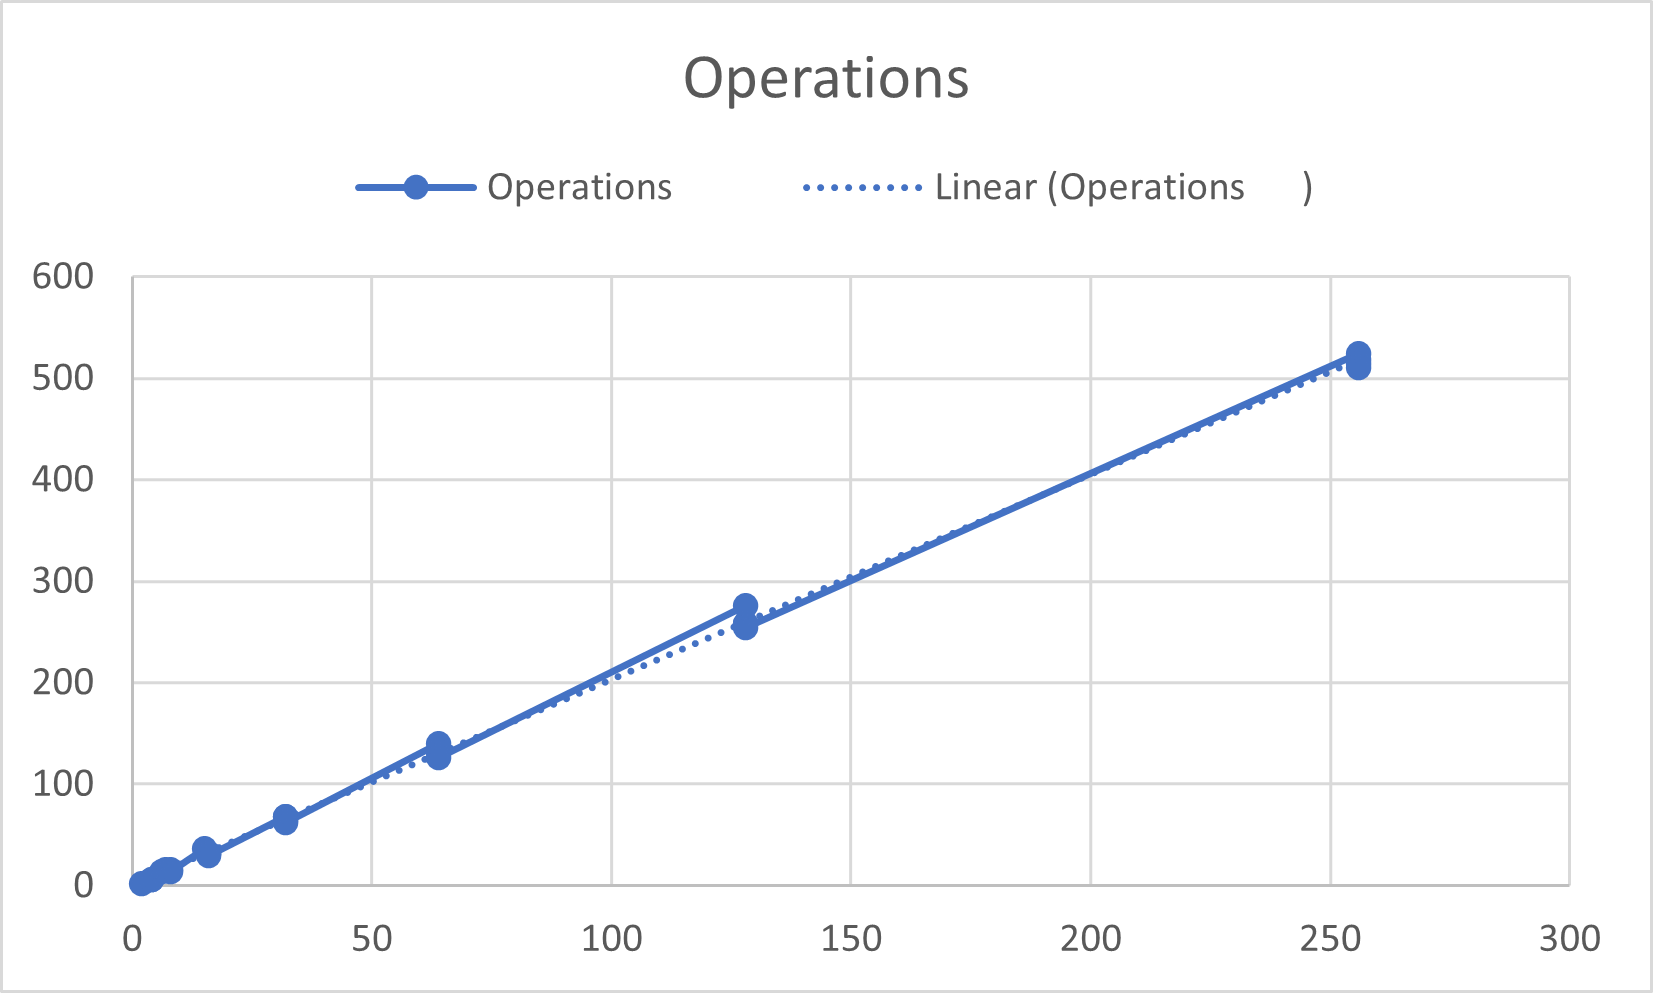
\includegraphics[width=8cm]{Greedy Algorithm/Operations.png}
    \caption{Greedy Algorithm Operations}
\end{figure}

\begin{figure}[H]
    \centering
    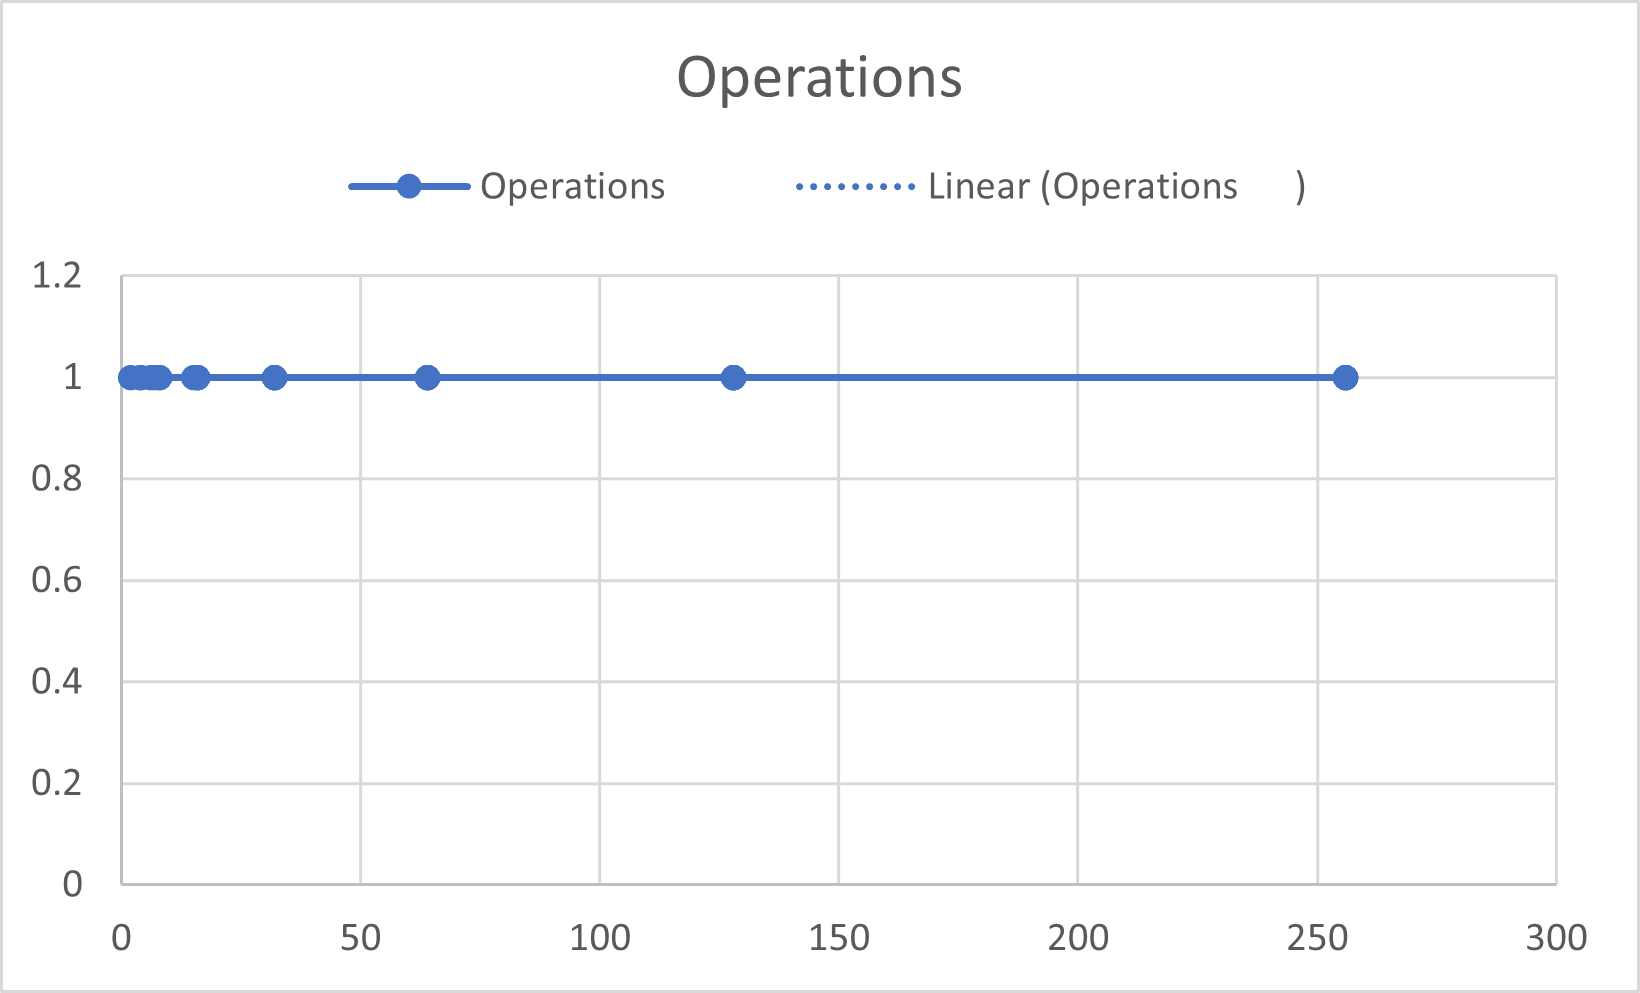
\includegraphics[width=8cm]{Breadth-First/Operations.png}
    \caption{Breadth-First Search Basic Operations}
\end{figure}

As we can evaluate from the previous graphs, the empirical analysis matches what was stated in the formal analysis:
\begin{itemize}
\item The exhaustive algorithm's order of growth is exponential.
\item The greedy algorithm's order of growth is linear.
\item The breadth-first search' order of growth is linear (constant).
\end{itemize}


\subsection{Solutions Tested}

\begin{figure}[H]
    \centering
    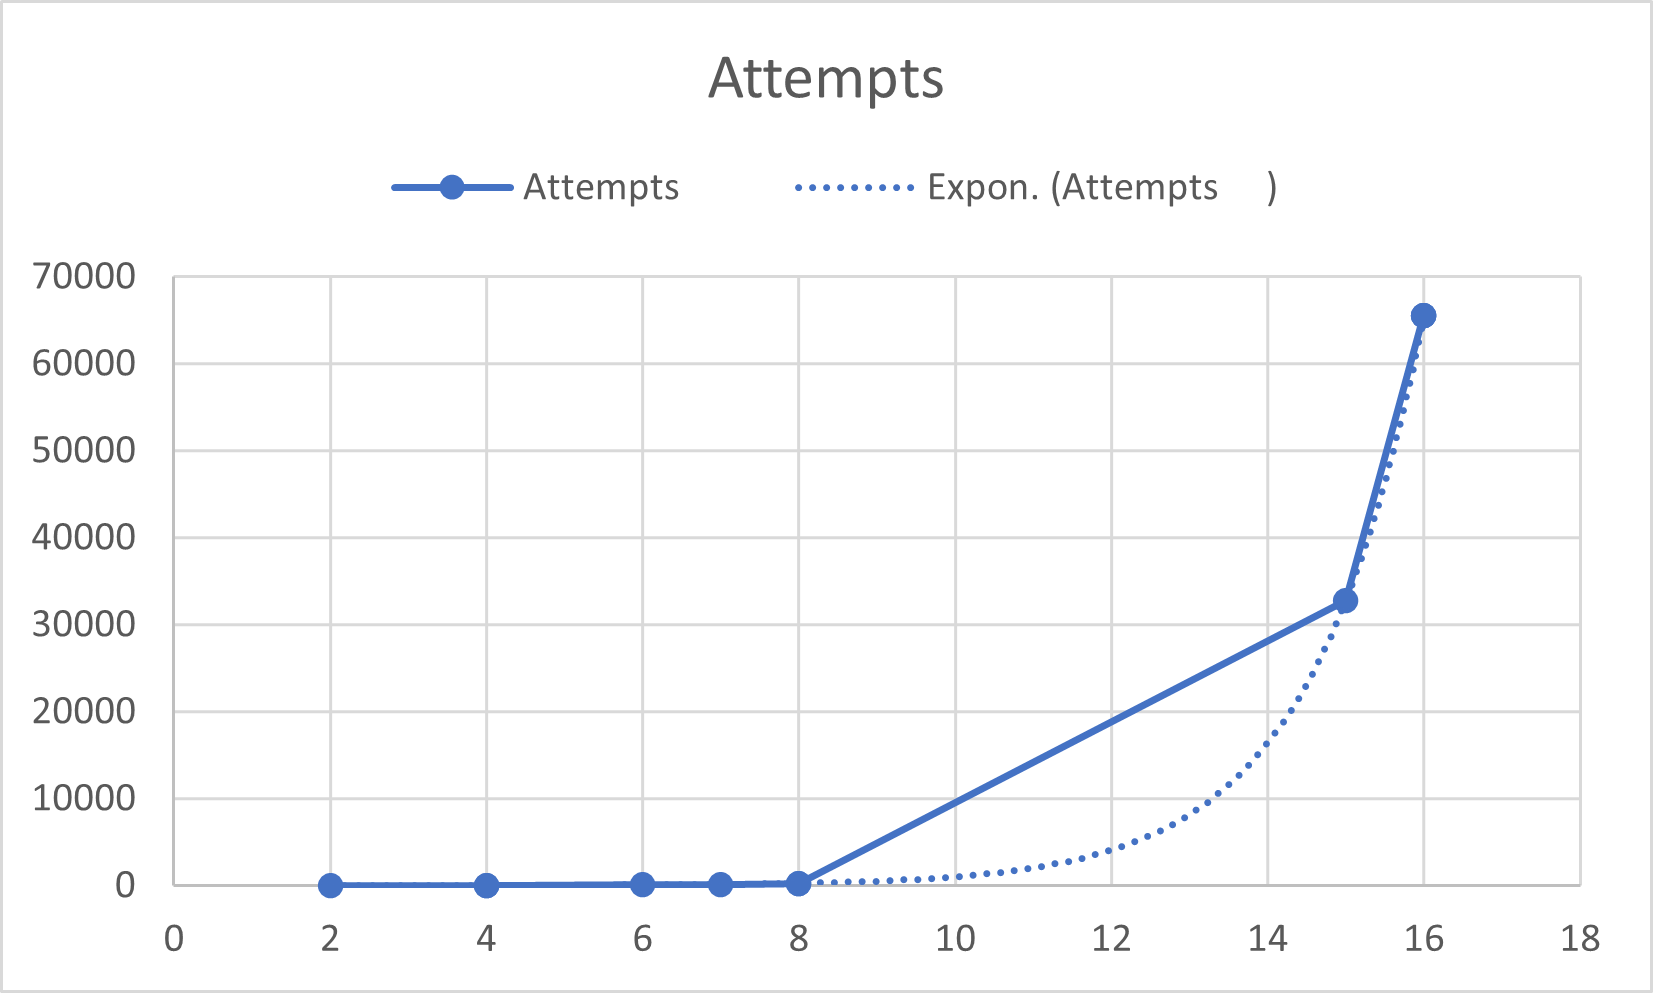
\includegraphics[width=8cm]{Exhaustive Search/Attempts.png}
    \caption{Exhaustive Search Attempts}
\end{figure}

\begin{figure}[H]
    \centering
    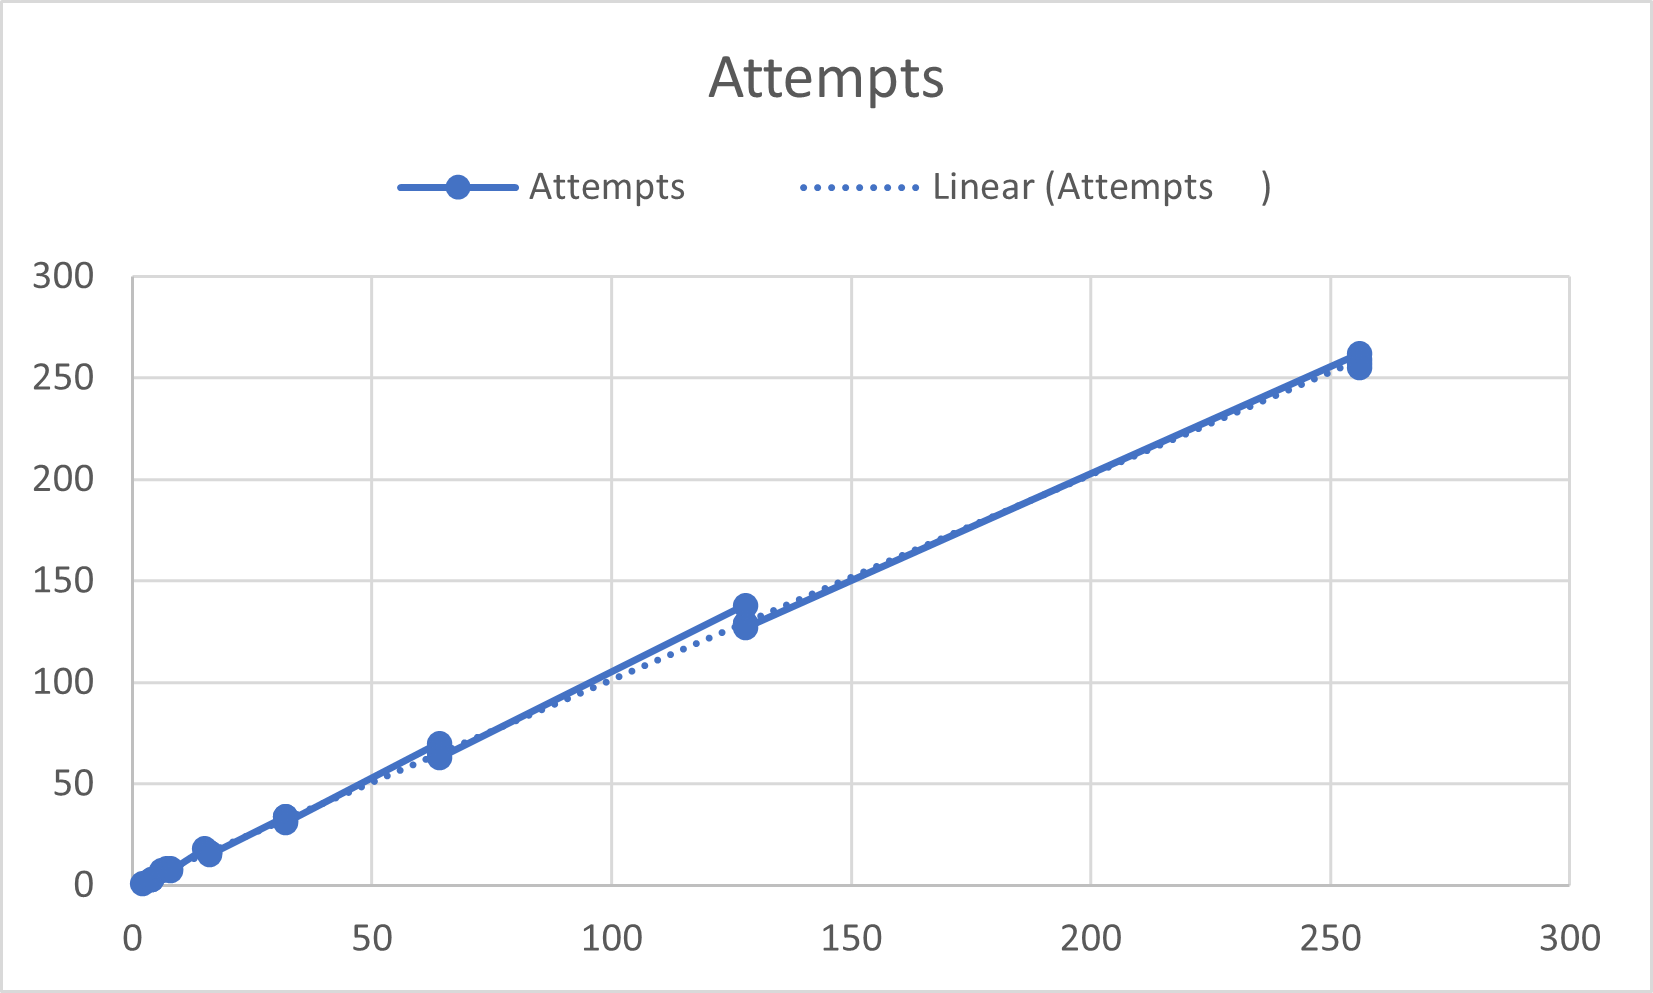
\includegraphics[width=8cm]{Greedy Algorithm/Attempts.png}
    \caption{Greedy Algorithm Attempts}
\end{figure}

\begin{figure}[H]
    \centering
    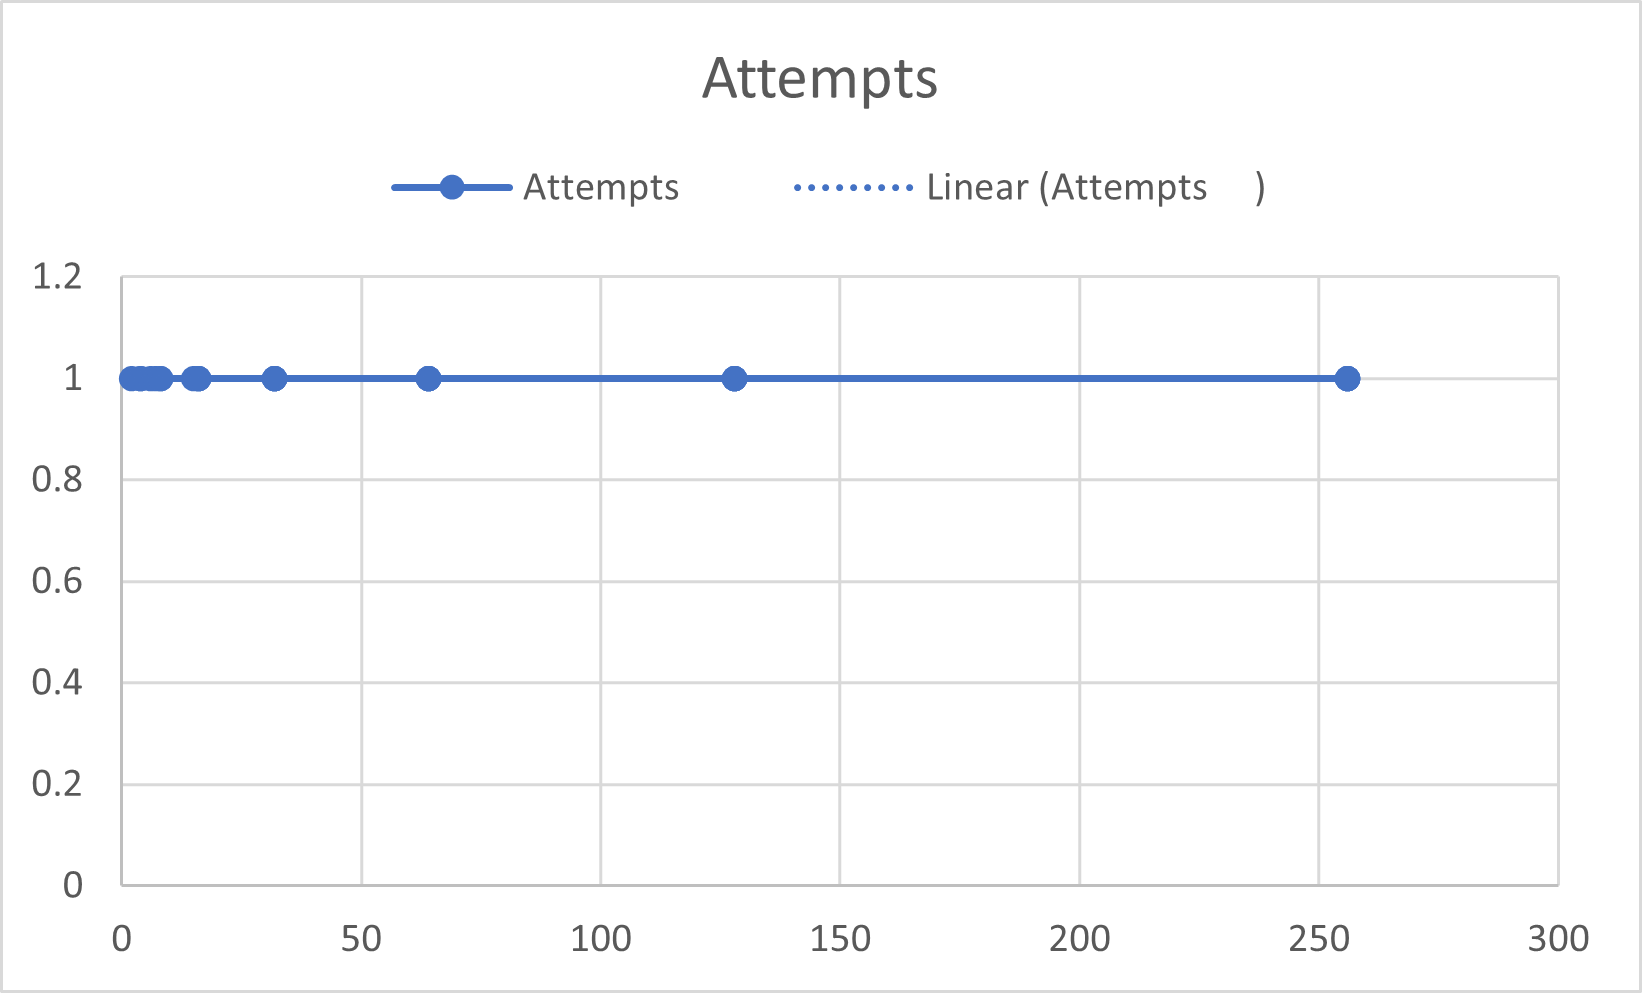
\includegraphics[width=8cm]{Breadth-First/Attempts.png}
    \caption{Breadth-First Search Attempts}
\end{figure}

Once again, we were able to prove empirically what we concluded in the formal analysis:
\begin{itemize}
\item For the exhaustive search and breadth-first search algorithms, the number of solutions tested is the same as the number of basic operations.
\item For the greedy search algorithms, the number of solutions tested is half the number of basic operations (since we perform two basic operations per solution tested).
\end{itemize}

\subsection{Execution Time}

\begin{figure}[H]
    \centering
    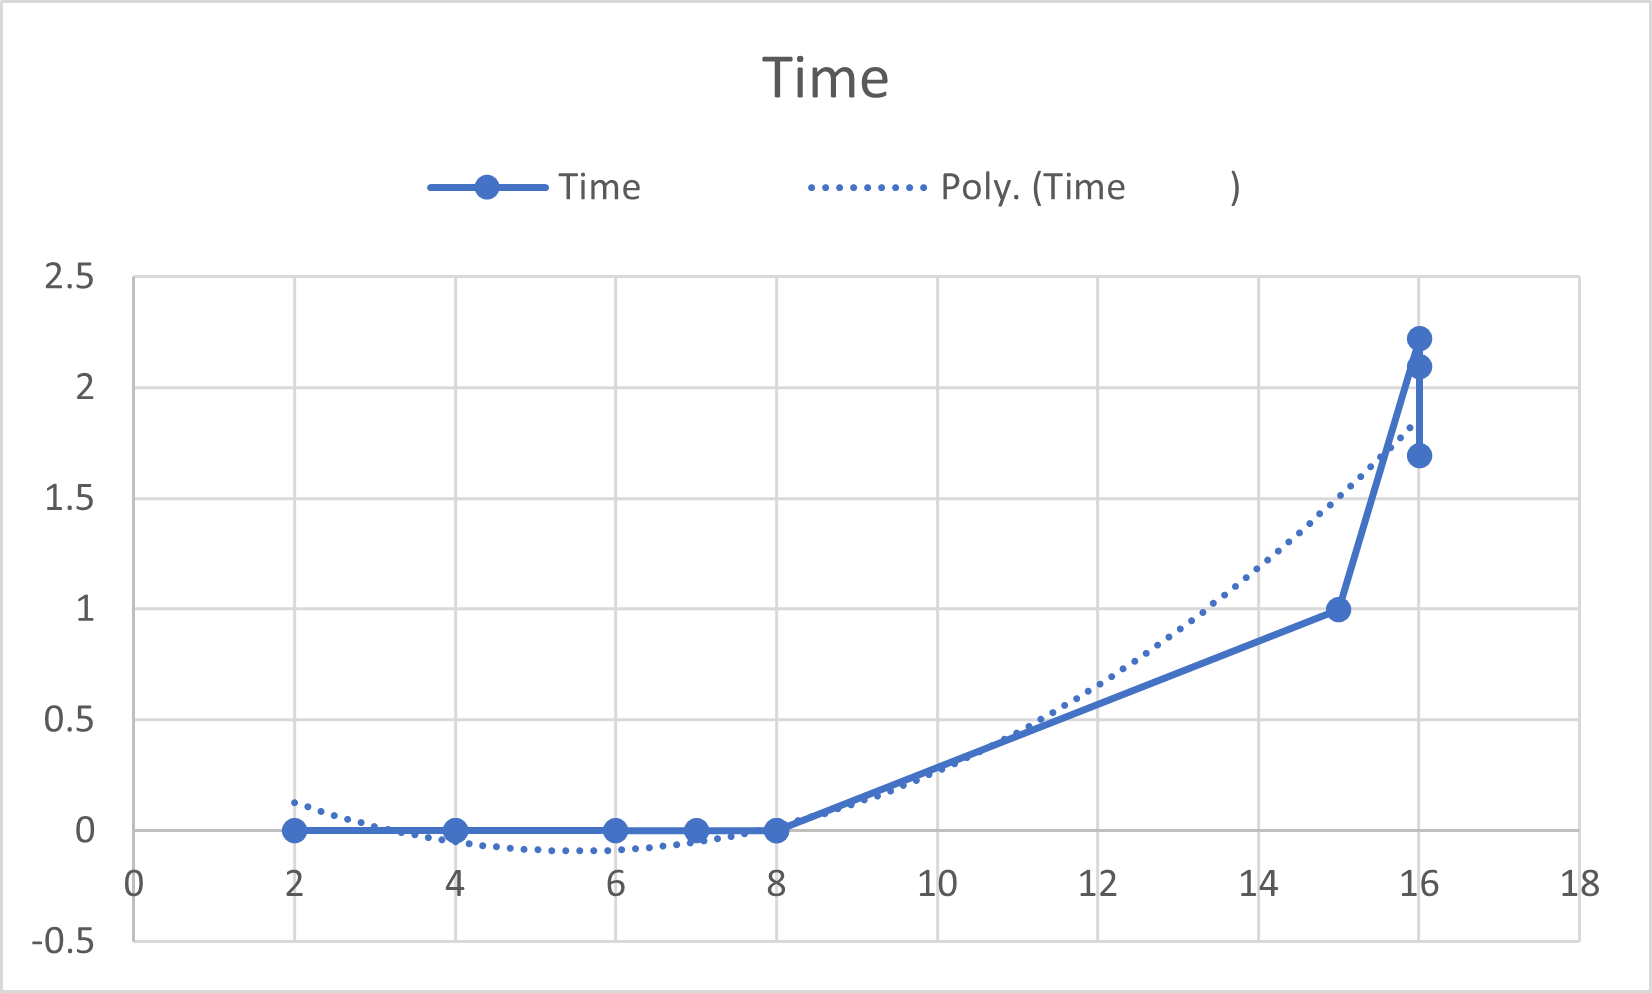
\includegraphics[width=8cm]{Exhaustive Search/Time.png}
    \caption{Exhaustive Search Execution Time}
\end{figure}

\begin{figure}[H]
    \centering
    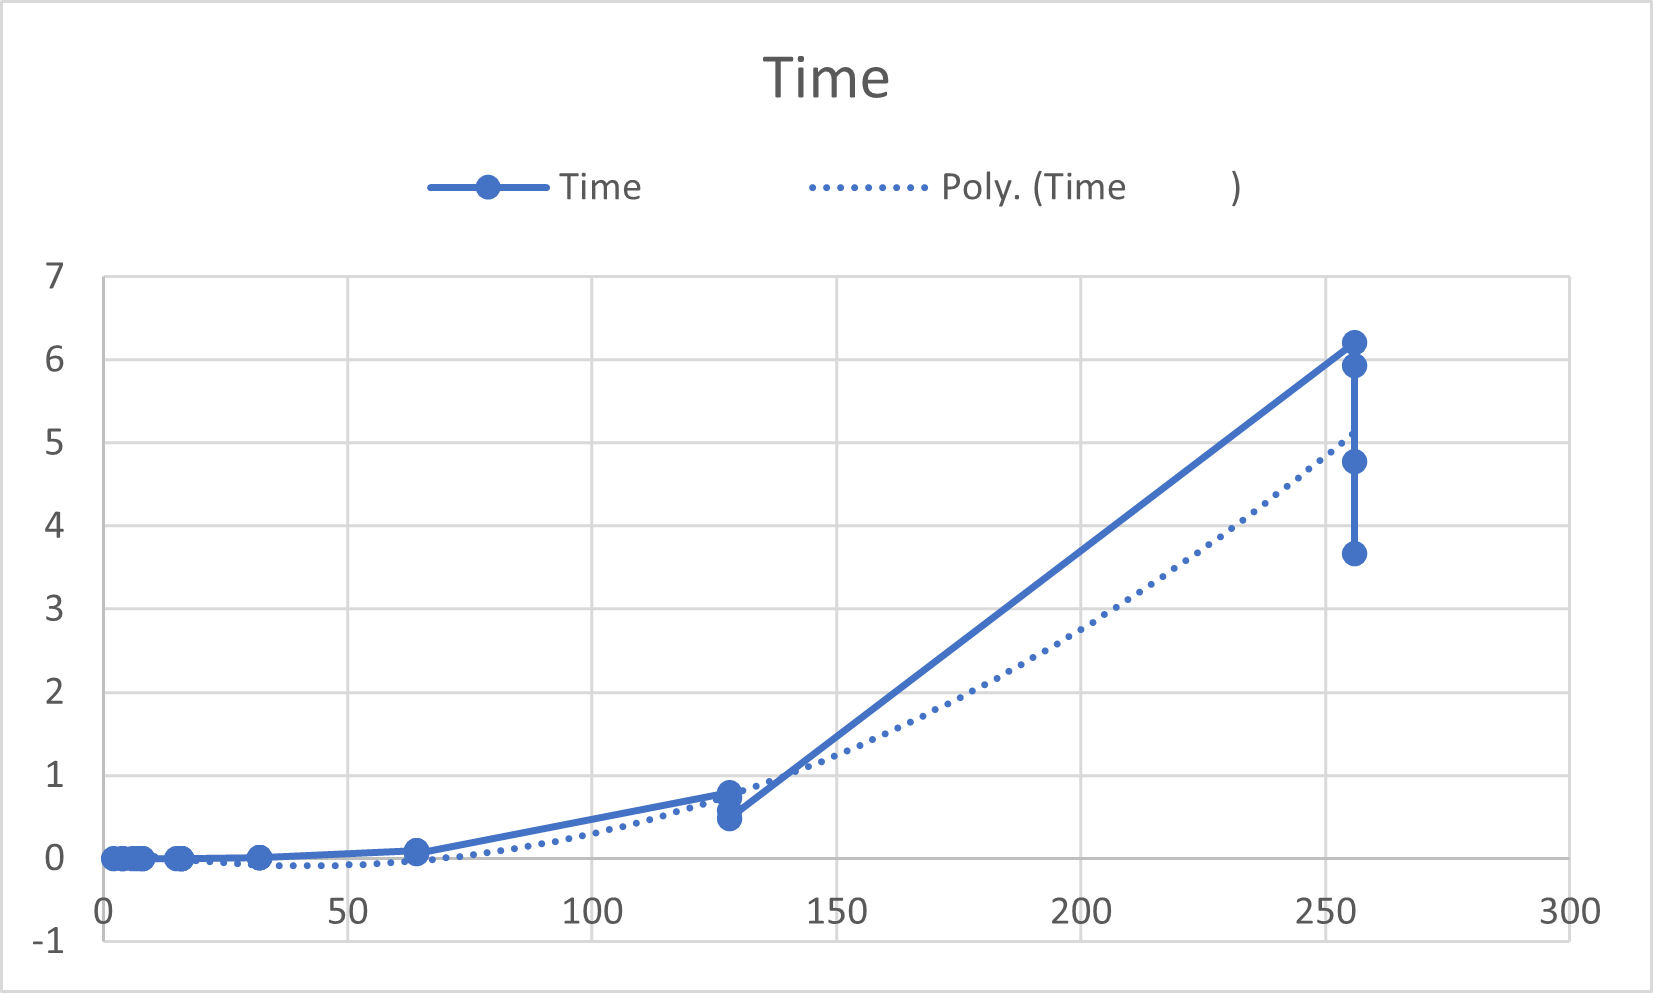
\includegraphics[width=8cm]{Greedy Algorithm/Time.png}
    \caption{Greedy Algorithm Execution Time}
\end{figure}


\begin{figure}[H]
    \centering
    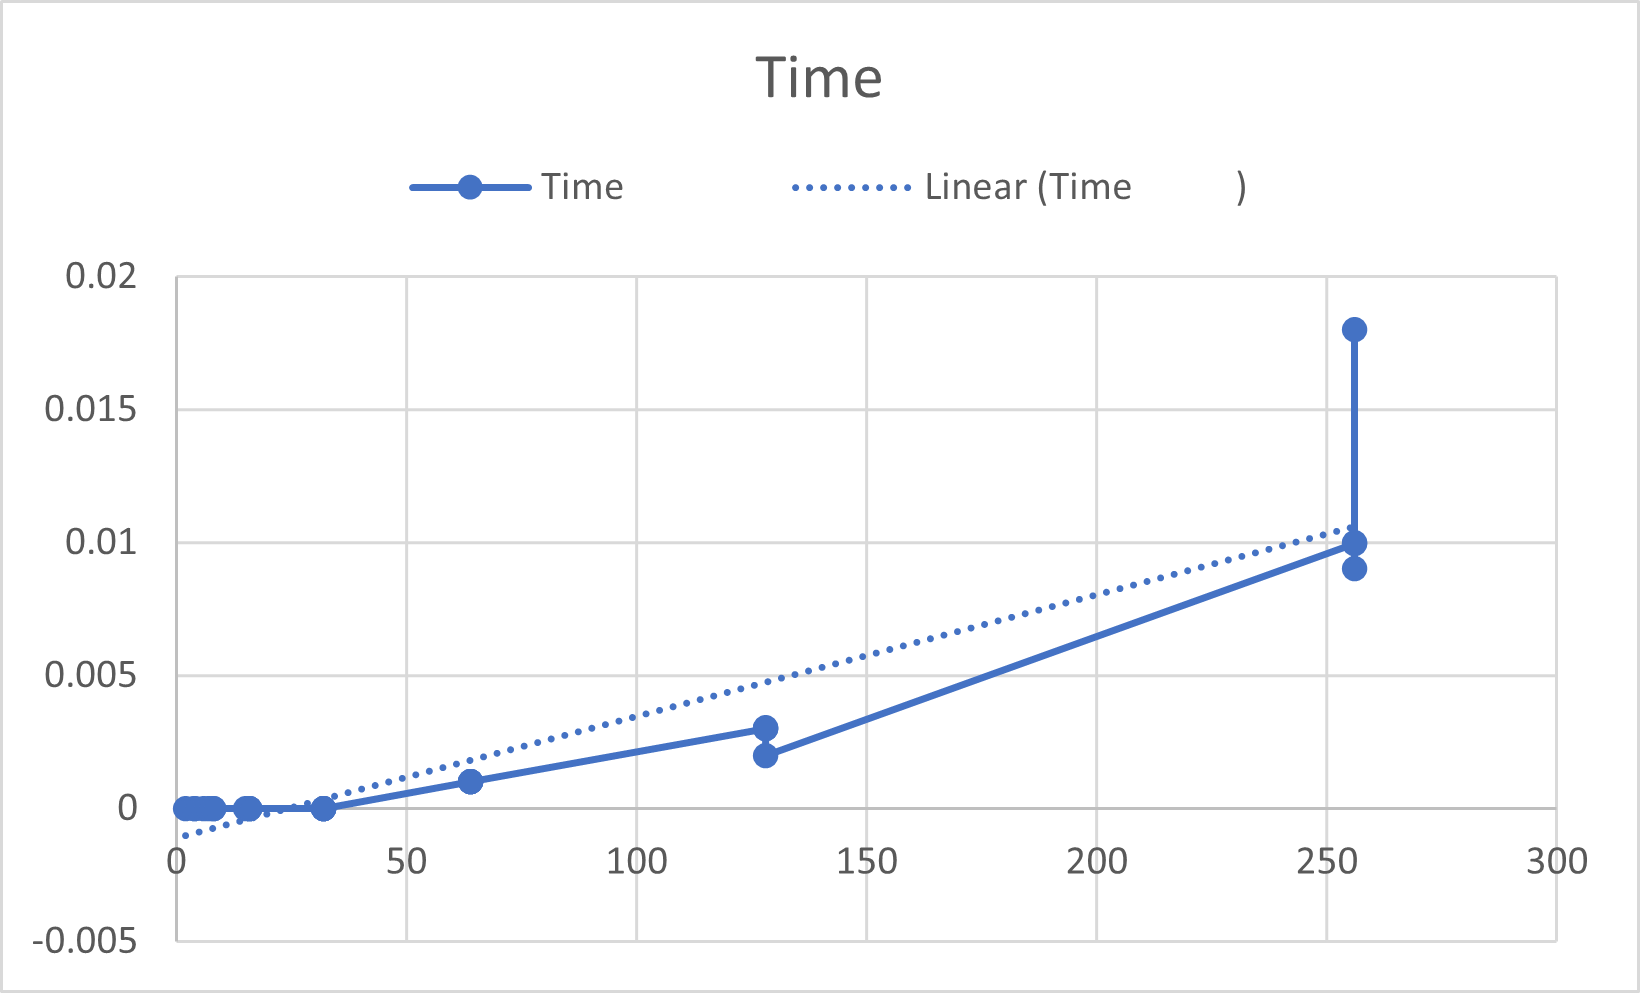
\includegraphics[width=8cm]{Breadth-First/Time.png}
    \caption{Breadth-First Search Execution Time}
\end{figure}

Finally, we proved that the execution time (in seconds) is not a good measurement of running time, as it produces different results for the same input of size n and for the same number of executed operations.

\section{Conclusion}

To conclude this document, we now understand that, as expected, an exhaustive search approach to this problem is very costly (with exponential computational complexity). The first greedy approach developed also showed to be costly (in particular, time-wise) and a poor choice for optimal or near-optimal results. However, the second greedy approach, breadth-first search, is an example that the simplest algorithms can, at times, produce optimal results without the cost of high computation complexity.

\begin{thebibliography}{00}

\bibitem{b1} Wikipedia (2022). \textit{Maximum cut} [Online]. Available: \url{https://en.wikipedia.org/wiki/Maximum_cut}
\bibitem{b2} Shiva Basava P. \textit{Maximum cut Problem} [Online]. Available: \url{https://iq.opengenus.org/maximum-cut-problem}
\bibitem{b3} Debmalya Panigrahi (2015). \textit{COMPSCI 532: Design and Analysis of Algorithms} [Online]. \url{https://courses.cs.duke.edu/cps232/fall15/scribe_notes/lec17.pdf}

\end{thebibliography}

\end{document}
